\documentclass[11pt,a4paper]{article}
\usepackage{booktabs}
\usepackage{graphicx}
\usepackage{times}
\usepackage{latexsym}
\renewcommand{\UrlFont}{\ttfamily\small}

\usepackage{microtype}

\title{\textbf{Interactive Natural Language Inference Classification }
}

\author{Shira Rozenthal \\
  Tulane University / New York City, NY \\
  \texttt{shira.rozenthal@gmail.com} \\
  \and
  Peter Sapountzis \\
  Tulane University / San Francisco, CA \\
  \texttt{peter.sapountzis@gmail.com}
}

\date{}

\begin{document}
\maketitle
\begin{abstract}
This study introduces an enhanced approach to Natural Language Inference (NLI) classification, leveraging the advanced mDeBERTa-v3-base-xnli-multilingual-nli-2mil7 model to categorize textual relationships across diverse linguistic contexts. Our project centers on the MultiNLI (MNLI) dataset, which spans a broad spectrum of text genres, including both written and spoken forms, sourced from various real-world documents and conversations. By incorporating this dataset, we address the challenge of classifying relationships into entailment, contradiction, or neutrality, which is essential for applications like automated reasoning and information extraction.

\\~\\

We augmented the mDeBERTa model, originally pre-trained on the CC100 multilingual dataset, to improve its application in zero-shot multilingual classification tasks, thus enhancing its adaptability and performance across unseen genres. Experimental results demonstrate that our modified mDeBERTa model achieves a validation accuracy of up to 85\%, indicating robust performance in NLI tasks across multiple languages. Qualitative assessments also revealed that the model adeptly handles a variety of text inputs, though it occasionally struggles with ambiguous or sarcastically framed texts.

\end{abstract}

\pagebreak 

\section{Introduction}
Natural Language Inference (NLI) is a machine learning task that determines the logical relationship between two text sequences. NLI is pivotal for understanding textual relationships and categorizing them into entailment, contradiction, or neutrality. As undergraduates, our interest in NLI stems from its foundational role in understanding and processing human language, which is critical for applications like fact-checking without a premise.

\

For example, the premise “Peter and Shira are at the Tulane library working on this project”

\

\textbf{\textit{Entails }}that Peter and Shira are students

\textbf{\textit{Contradicts }}that Peter and Shira are asleep

Is \textbf{\textit{neutral }}on whether they are having fun

\

...(we're having fun we promise!) Our goal with this project is to explore the world of textual entailment by diving into the challenge of classifying premise/hypothesis relationships across a wide range of written and conversational contexts. 

\\~\\

\section{Related Work}

\

\begin{itemize}
    \item \textbf{A large annotated corpus for learning natural language }
\end{itemize}
This paper introduces the SNLI corpus, providing a foundational dataset for NLI research.

\
\
\

\begin{itemize}
    \item \textbf{A Broad-Coverage Challenge Corpus for Sentence Understanding through Inference }
\end{itemize}
This paper introduces the MNLI corpus, the second largest NLI dataset available for use.

\
\

\begin{itemize}
    \item \textbf{BERT: Pre-training of Deep Bidirectional Transformers for Language Understanding }
\end{itemize}
This paper provides a new approach to generating deep contextualized word representations,                   which have significantly improved performance on a variety of NLP tasks, including NLI. Its                      methodology for pre-training on a large corpus and fine-tuning for specific tasks provides a robust          framework that we can apply and adapt to enhance our NLI model's ability to understand and                  infer the relationships between sentence pairs with greater accuracy.
    
\
\

\begin{itemize}
    \item \textbf{Adversarial NLI: A New Benchmark for Natural Language Understanding}
\end{itemize}
This paper introduces the ANLI dataset, a meticulously curated collection designed to challenge                NLU systems with adversarially crafted examples. This benchmark is crucial for evaluating the                 robustness of NLI models against complex linguistic phenomena and nuanced inference challenges         that are not well-represented in existing datasets. The introduction of ANLI underscores the                      importance of adversarial testing in revealing the limitations of current models and guiding the               development of more sophisticated, resilient NLU systems, making it a pivotal reference for                       projects aiming to enhance NLI methodologies.

\
\
\

\begin{itemize}
    \item \textbf{IMPLI : Investigating NLI Models’ Performance on Figurative LanguageLinks to an external site. }
\end{itemize}
This paper introduces the IMPLI dataset, focusing on the underexplored area of how NLI models handle figurative language, such as idioms and metaphors. It is highly relevant to our project as it presents a novel benchmark for evaluating the capability of NLI systems to understand and interpret figurative speech—an aspect that traditional datasets may overlook. By demonstrating that even advanced models like RoBERTa fine-tuned on MNLI struggle with non-entailing pairs in this context, the paper underscores a significant gap in current NLI methodologies


\\~\\

\section{Methods}
We are working with one of the leading datasets in this space, the MultiNLI (MNLI) dataset.

MNLI extends the concept of the SNLI dataset by incorporating a wider variety of text, including both spoken and written forms across ten different genres sourced from the Open American National Corpus.

These genres include transcriptions of face- to-face conversations, government documents, letters related to philanthropic fundraising, the 9/11 Commission report, non-fiction works published by Oxford University Press, articles from Slate Magazine, telephone conversations, travel guides, linguistics posts, and contemporary fiction. For each premise drawn from these sources, crowdworkers generated three new sentences to represent entailment (statements that are necessarily true if the premise is true), contradiction (statements that are necessarily false), and neutral (where neither condition applies). A distinctive aspect of MNLI is that only half of the genres are included in the training set, with the remaining unseen genres serving to test a model's ability to generalize to new text sources.

We are utilizing the mDeBERTa-v3-base-xnli-multilingual-nli-2mil7 model. This model is an advanced multilingual model capable of performing natural language inference (NLI) across 100 languages, making it highly suitable for multilingual zero-shot classification tasks. Developed by Microsoft, it is based on the mDeBERTa-v3-base architecture and has been pre-trained on the CC100 multilingual dataset, which encompasses text in 100 languages.

\\~\\

\section{Experiment}
We focused on optimizing our model's training process to achieve a balance between performance and efficiency. 

We began by determining the optimal subset to train: Our model is pre-trained on natural language data, and we aim to refine it further using a carefully selected subset of training data. The goal is to observe at what point the validation accuracy plateaus, indicating diminishing returns on further training. This allows us to optimize runtime without compromising model performance.

We utilized a 4-epoch training loop for our model, focusing on an efficient integration of techniques like gradient clipping to manage the stability of training dynamics. Our training involved processing batches of data, where each batch was moved to a GPU to harness accelerated computing capabilities. The loss for each batch was computed based on the model's outputs and then used for backpropagation.

To mitigate the exploding gradient problem—a common issue in training deep neural networks—we implemented gradient clipping. This technique caps the gradients during backpropagation to a maximum norm of 1.0, ensuring that updates to the model parameters remain small and manageable, thus maintaining the stability of the model throughout the training process.

After computing the gradients, we updated the model's weights using AdamW. This was accompanied by a scheduler that dynamically adjusted the learning rate, aimed at reducing it as the epochs progressed to allow the model to settle into a more stable and possibly optimal convergence region. Throughout each epoch, we maintained a running total of the loss, which was displayed via a progress bar. This real-time feedback allowed us to monitor the model's training performance and adjust parameters if necessary.

In the validation phase, the model was set to evaluation mode, which disables specific layers/functions like dropout, making the model's behavior consistent and deterministic. We evaluated the model on a separate validation dataset to ensure that our metrics reflected the model's ability to generalize to unseen data.

For each batch in the validation set, we computed the logits, which were then used to derive predictions by selecting the class with the highest logit value as the most likely label. Accuracy for each batch was calculated by comparing these predictions to the true labels, with the mean accuracy across all batches giving us a measure of overall model performance.
\\~\\
\textbf{Results and Observations}: From the training process, we observed that the average loss consistently decreased across epochs, indicating effective learning.The model demonstrates solid quantitative performance metrics, with a maximum attained validation accuracy of 85\%. Qualitative evaluations highlight its robustness in handling various text inputs. Notably, this model showed particular strength in scenarios involving clear semantic boundaries but faced challenges with nuanced or context-dependent texts. Stress testing revealed some issues in handling ambiguous or sarcastic texts, leading to misinterpretations. 

For example, in reference to Figures 2 and 3 in section 6, the model handles the following instances “I’m studying” and “My phone is dead” well, classifying the relationship between the two as neutral with 99.98\% confidence. In Figure 3, however, simply interchanging “low battery” with “dead” throws it off, as it misclassifies to contradiction with similarly high confidence levels. 


\\~\\

\section{Conclusion}

As we reflect on this project, it stands out as a tremendous learning opportunity, especially in applying theoretical knowledge in the field of Natural Language to practical, real-world challenges we’ve encountered in our personal uses of generative language models. 

Looking forward, there is ample room for extending this research. Future endeavors could focus on enhancing the model's sensitivity to linguistic subtleties by incorporating a broader spectrum of semantic analysis tools or by training on a more diverse dataset that includes a wider array of informal texts. Additionally, exploring the integration of context-aware algorithms could potentially mitigate the biases towards certain text genres, paving the way for more universally applicable NLI systems. 

\\~\\
\section{Screenshots}
\pagebreak 

\begin{figure}
    \centering
    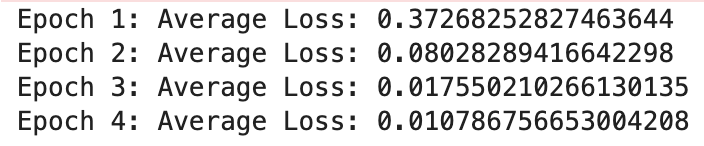
\includegraphics[width=1\linewidth]{Epochs.png}
    \caption{Model Performance}
    \label{fig:enter-label}
\end{figure}
\begin{figure}
    \centering
    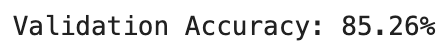
\includegraphics[width=1\linewidth]{ValAccuracy.png}
    \caption{Model Performance}
    \label{fig:enter-label}
\end{figure}

\begin{figure}
    \centering
    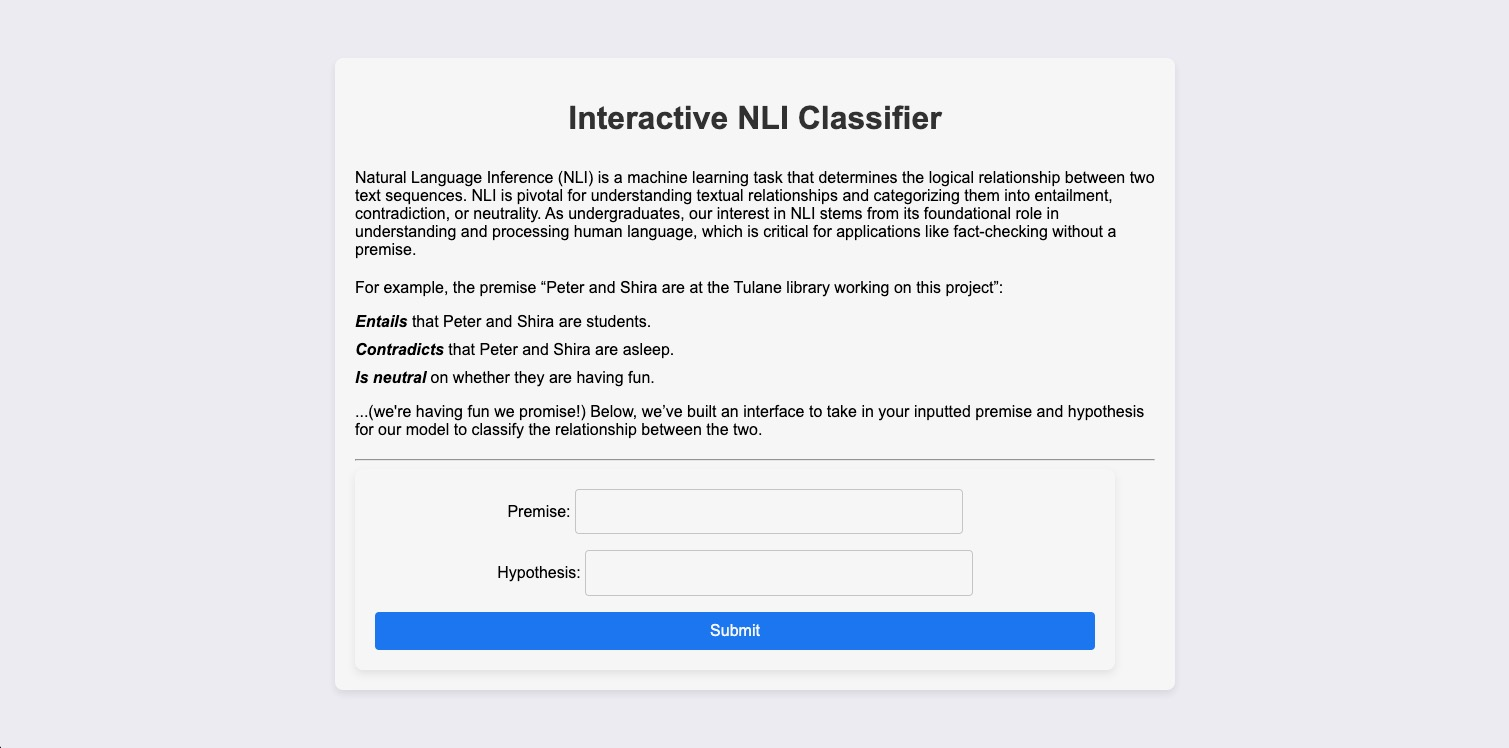
\includegraphics[width=1\linewidth]{Interface.jpeg}
    \caption{User Interface}
    \label{fig:enter-label}
\end{figure}
\begin{figure}
    \centering
    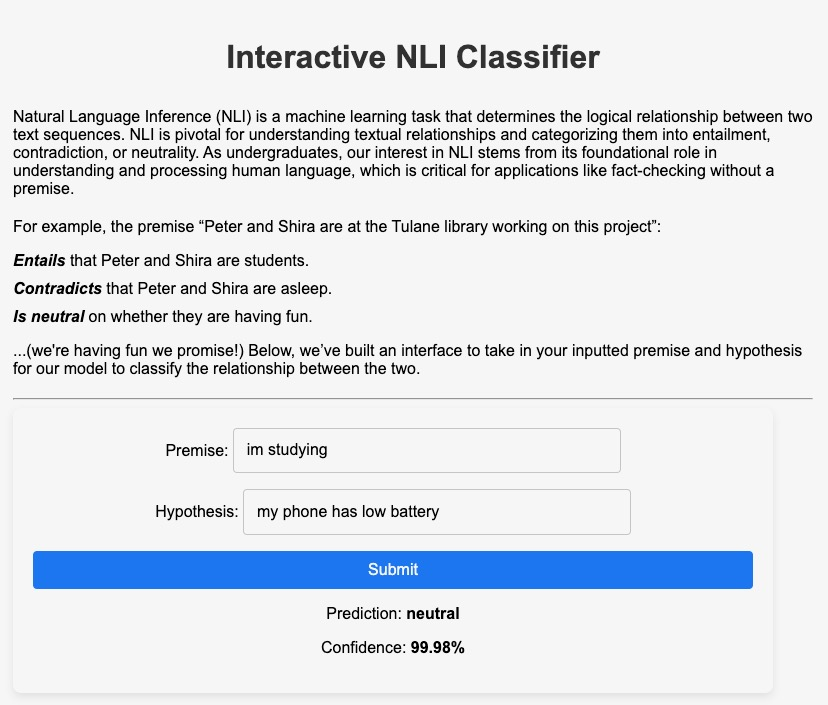
\includegraphics[width=0.75\linewidth]{Example1.jpeg}
    \caption{correctly classified with 99.98 percent confidence}
    \label{fig:enter-label}
\end{figure}
\begin{figure}
    \centering
    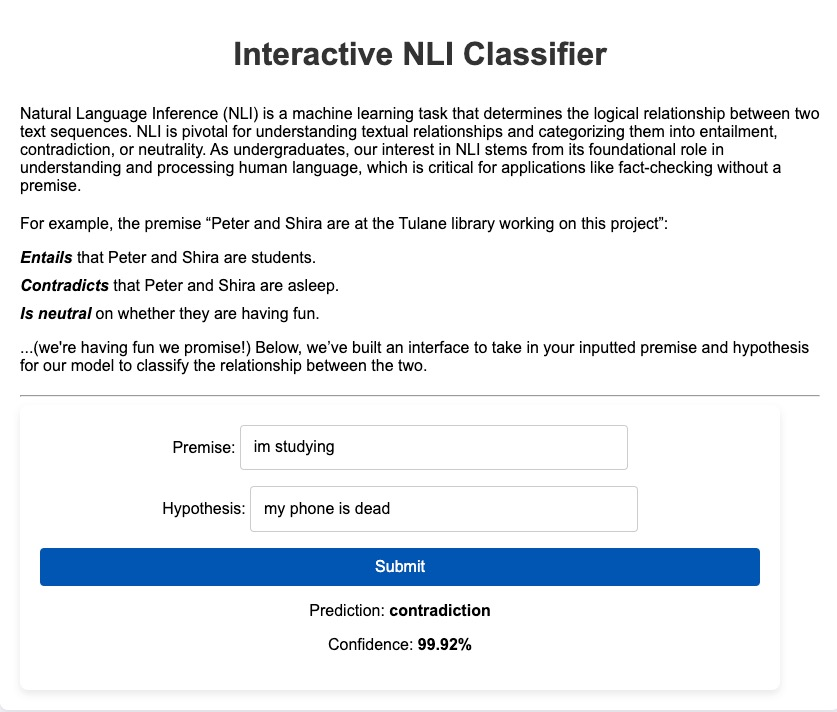
\includegraphics[width=0.75\linewidth]{Example2.jpeg}
    \caption{misclassified with 99.92 percent confidence when "low battery" gets interchanged with "dead"}
    \label{fig:enter-label}
\end{figure}
\end{document}